\documentclass[11pt]{article}
\usepackage{graphicx}

\begin{document}
\title{Homework 3}
\author{Colt Bradley}
\date{}
\maketitle

\section{Equations and Plot}
The goal of this lesson was to import modules to solve and graph simple physics problem. For this homework, the problem in question was a projectile problem. Given an initial velocity $v_0$ at an initial angle $\theta$, we needed to calculate the x and y coordinates of the projectile. After solving the equation $\vec F = m\vec a$ for each of x and y direction, you get

\begin{equation}
y = v_y t - \frac{1}{2} g t^2
\end{equation}
\begin{equation}
x = v_x t
\end{equation}
Where
\begin{equation}
v_x = v_0 Cos(\theta)
\end{equation}
\begin{equation}
v_y = v_0 Sin(\theta)
\end{equation}

For $v_0 = 20 \frac{m}{s}$ and $\theta = 45^{\circ}$, the plot follows:
\begin{figure}[ht]
\centering
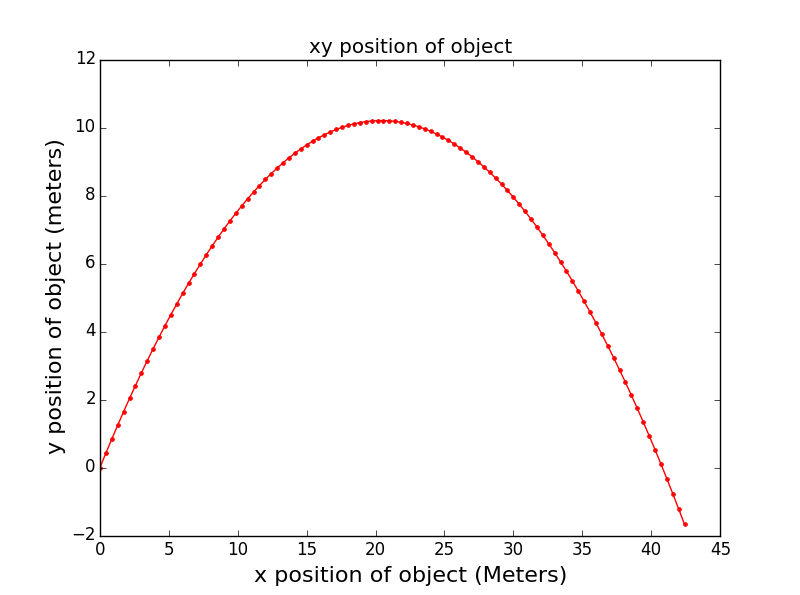
\includegraphics[scale=.4]{xy_projectile.png}
\end{figure}

\section{Code}
\begin{verbatim}
#Colt Bradley
#1.18.16
#Homework for Lesson 3

#Import modules numpy for mathy stuff and pylab for plots
import numpy as n
import pylab as p

#Ask user for initial velocity and theta
v0 = raw_input("Initial Velocity: ")
v0 = float(v0)
theta = raw_input("Initial Angle: ")
theta = float(theta)

#Import parameters and convert user-given values
theta = n.pi*theta/180
vy = v0*n.sin(theta)
vx = v0*n.cos(theta)
g = 9.8
t = n.linspace(0.,3.,100)

#Essential equations
x = vx*t
y = vy*t - .5*g*t**2

#plot commands
p.plot(x,y,"r")
p.plot(x,y,"r.")
#plot labels
p.title("xy position of object")
p.xlabel("x position of object (Meters)",fontsize=16)
p.ylabel("y position of object (meters)",fontsize=16)
p.show()
p.savefig("xy_projectile.png")
\end{verbatim}


\end{document}